\subsubsection{Tiến trình Thu thập Dữ liệu}
Nội dung trọng tâm được triển khai trong phần này là xây dựng cơ chế thu thập thông tin khí hậu chính xác từ cảm biến kỹ thuật số DHT20. Sau quá trình thu thập dữ liệu, tất cả những thông tin về nhiệt độ và độ ẩm sẽ được lưu trữ trong Message Queue. Từ đấy toàn bộ dữ liệu sẽ được hệ thống phân tích và biểu diễn đa dạng thông qua các giao diện phần cứng khác nhau: từ việc hiển thị ký tự trên màn hình LCD cho đến việc sử dụng các trạng thái ánh sáng của LED đơn và LED RGB, qua đó tạo ra một hệ thống trực quan hóa dữ liệu sinh động và dễ dàng quan sát.

\subsubsection{Hiển thị trên LED đơn với các trạng thái nhiệt độ khác nhau}
Tác vụ quản lý thiết bị hiển thị LED đơn chịu trách nhiệm biểu diễn trạng thái nhiệt độ thông qua các nhịp điệu chớp tắt khác nhau. Hệ thống phân loại điều kiện môi trường dựa trên kiểu liệt kê \texttt{LEDBlinkyState\_t} với năm cấp độ riêng biệt. Mỗi cấp độ sẽ tương ứng với một khoảng thời gian được bộ định thời của hệ điều hành quản lý chặt chẽ nhằm đảm bảo tính chính xác về mặt thời gian thực.


\begin{figure}[H]
    \centering
    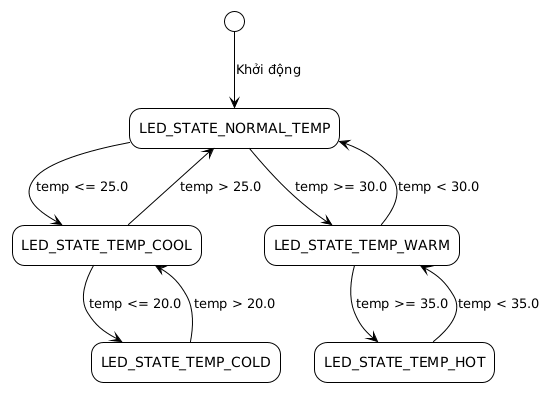
\includegraphics[width=1\textwidth]{pictures/FSM_LED.png}
    \caption{FSM các trạng thái của LED đơn tương ứng với từng mức nhiệt độ}
\end{figure}


\begin{itemize}
    \item \textbf{\texttt{LED\_STATE\_TEMP\_HOT}:} Trạng thái này xuất hiện khi nhiệt độ đo được vượt ngưỡng 35$^\circ$C. Để cảnh báo tình trạng quá nhiệt nghiêm trọng, đèn LED sẽ được điều khiển chớp tắt với tần suất cực nhanh là 100 mili giây cho mỗi chu kỳ.
    \item \textbf{\texttt{LED\_STATE\_TEMP\_WARM}:} Khi nhiệt độ nằm trong khoảng từ 30$^\circ$C đến dưới 35$^\circ$C, hệ thống xác định đây là vùng cảnh báo mức độ thấp. Nhịp điệu của đèn LED lúc này được duy trì ổn định ở mức 300 mili giây.
    \item \textbf{\texttt{LED\_STATE\_NORMAL\_TEMP}:} Đây là dải nhiệt độ lý tưởng cho vận hành, được xác lập khi giá trị đo được nằm giữa 25$^\circ$C và 30$^\circ$C. Đèn LED duy trì nhịp chớp tắt tiêu chuẩn là 1000 mili giây để biểu thị hệ thống đang hoạt động trong điều kiện bình thường.
    \item \textbf{\texttt{LED\_STATE\_TEMP\_COOL}:} Trong trường hợp môi trường trở nên mát mẻ hơn với nhiệt độ từ trên 20$^\circ$C đến 25$^\circ$C, hệ thống sẽ chuyển sang trạng thái này. Tần suất hoạt động của đèn sẽ chậm lại đáng kể với chu kỳ là 2000 mili giây.
    \item \textbf{\texttt{LED\_STATE\_TEMP\_COLD}:} Đây là mức nhiệt độ thấp nhất khi giá trị xuống dưới hoặc bằng 20$^\circ$C. Hệ thống phát tín hiệu bằng cách chớp tắt LED rất chậm với khoảng thời gian lên đến 3000 mili giây giữa các lần chuyển đổi trạng thái.
\end{itemize}

Ngoài ra, việc điều khiển chân tín hiệu của LED còn chịu ảnh hưởng trực tiếp từ tín hiệu RPC được gửi từ app.coreiot.io. Các tín hiệu đó sẽ làm thay đổi \texttt{xSemaphoreLedControl}. Chỉ khi lấy được thành công Semaphore này, hệ thống cho phép LED hoạt động dựa trên logic thời gian như trên và sau đó hoàn trả quyền điều khiển. Ngược lại nếu không lấy được Semaphore, đèn LED đơn sẽ bị ép về trạng thái tắt.

\subsubsection{Hiển thị RGB LED tương ứng với các trạng thái độ ẩm khác nhau}
Phân hệ hiển thị đa sắc sử dụng dải RGB LED để cung cấp cái nhìn trực quan về độ ẩm không khí hiện tại và trạng thái mạng. Các trạng thái màu sắc được định nghĩa thông qua kiểu dữ liệu \texttt{NeoBlinkyState\_t} và phụ thuộc chặt chẽ vào độ ẩm hiện tại. Trong khi đó, trạng thái bật tắt của đèn sẽ do trạng thái kết nối mạng hiện tại quyết định.


\begin{figure}[H]
    \centering
    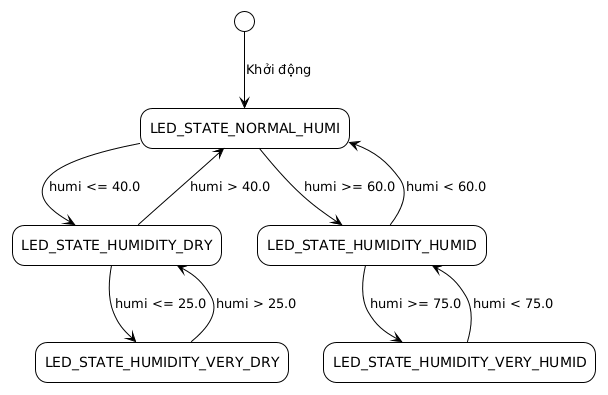
\includegraphics[width=1\textwidth]{pictures/FSM_NEO.png}
    \caption{FSM các trạng thái của RGB LED tương ứng với từng mức độ ẩm}
\end{figure}


\begin{itemize}    
    \item \textbf{Quản lý trạng thái kết nối:} Hệ thống ưu tiên kiểm tra cờ trạng thái của Semaphore kết nối mạng \texttt{xBinarySemaphoreInternet}. Nếu mất tín hiệu đường truyền, thiết bị sẽ phản hồi bằng cách cho dải LED chớp tắt liên tục mỗi 500 mili giây. Điểm đặc biệt là trong pha sáng, màu sắc vẫn phản ánh đúng mức độ ẩm hiện tại để người dùng không bị gián đoạn việc giám sát môi trường. Khi kết nối ổn định, dải LED sẽ chuyển sang chế độ sáng liên tục với màu sắc tương ứng.
    
    \item \textbf{Phân loại theo mức độ ẩm:} Màu sắc của dải LED được nội suy theo năm vùng giá trị cụ thể như sau:
    \begin{itemize}     
        \item \textbf{\texttt{LED\_STATE\_HUMIDITY\_VERY\_HUMID}:} Khi độ ẩm đạt mức rất cao từ 75\% trở lên, đèn chuyển sang màu Tím nhằm cảnh báo độ ẩm không khí các ở mức cao.
        \item \textbf{\texttt{LED\_STATE\_HUMIDITY\_HUMID}:} Với dải độ ẩm từ 60\% đến dưới 75\%, hệ thống hiển thị màu Lam để biểu thị môi trường đang ở mức khá ẩm ướt.
        \item \textbf{\texttt{LED\_STATE\_NORMAL\_HUMI}:} Màu Lục được chọn để biểu thị dải độ ẩm bình thường, dao động từ 40\% đến dưới 60\%.
        \item \textbf{\texttt{LED\_STATE\_HUMIDITY\_DRY}:} Khi không khí bắt đầu khô hanh với độ ẩm từ 25\% đến dưới 40\%, đèn sẽ chuyển sang màu Vàng để nhắc nhở người dùng.
        \item \textbf{\texttt{LED\_STATE\_HUMIDITY\_VERY\_DRY}:} Nếu độ ẩm rơi xuống mức cực thấp dưới 25\%, hệ thống lập tức hiển thị màu Đỏ để cảnh báo về điều kiện môi trường quá khô.
    \end{itemize}
\end{itemize}

\subsubsection{Hiển thị LCD}
Màn hình tinh thể lỏng đóng vai trò là trung tâm thông báo chi tiết của hệ thống. Dựa trên các thông số thu thập được, máy trạng thái của màn hình được điều khiển thông qua cấu trúc liệt kê \texttt{LCDState\_t} với ba chế độ hoạt động có tính phân cấp:

\begin{figure}[H]
    \centering
    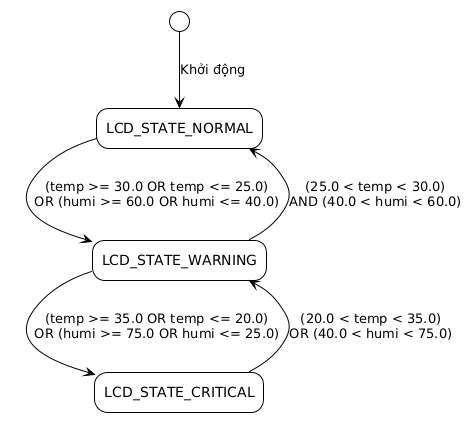
\includegraphics[width=1\textwidth]{pictures/FSM_LCD.png}
    \caption{FSM các trạng thái của LCD}
\end{figure}

\begin{itemize}
    \item \textbf{\texttt{LCD\_STATE\_NORMAL}:} Trong điều kiện môi trường ổn định, màn hình hiển thị trực tiếp các con số về nhiệt độ và độ ẩm một cách rõ ràng. Nội dung được định dạng lại để tối ưu hóa không gian hiển thị vốn hạn hẹp của các dòng ký tự, giúp người dùng nắm bắt nhanh các thông số cơ bản.
    \item \textbf{\texttt{LCD\_STATE\_WARNING}:} Khi một trong hai chỉ số môi trường bắt đầu rời khỏi vùng lý tưởng, hệ thống sẽ tự động chèn thêm thông điệp cảnh báo SOS ngay phía sau giá trị đo được. Việc này tạo ra một sự thay đổi trực quan trên giao diện hiển thị nhằm thu hút sự chú ý của người quan sát mà không làm mất đi các thông tin đo lường cần thiết.
    \item \textbf{\texttt{LCD\_STATE\_CRITICAL}:} Đây là trạng thái báo động cao nhất khi nhiệt độ hoặc độ ẩm chạm tới các ngưỡng cực đoan. Lúc này, màn hình sẽ chuyển sang chế độ nhấp nháy liên tục toàn bộ nội dung hoặc đèn nền. Sự thay đổi trạng thái thị giác mạnh mẽ này là phương thức cảnh báo cấp bách nhất, yêu cầu người vận hành phải có biện pháp can thiệp ngay lập tức để bảo vệ thiết bị hoặc điều chỉnh môi trường.
\end{itemize}


